\chapter{Desenvolvimento da Solução}

Este capítulo apresenta o desenvolvimento do Avaliador de Serviços Públicos a
partir dos artefatos da Lean Inception e da implementação do protótipo. O
desenvolvimento foi orientado pela hipótese de que o feedback contextual,
acionado no momento da dificuldade, pode gerar dados mais úteis do que uma
avaliação estática exibida apenas ao final da jornada.

\section{Visão Geral do Produto}

O Avaliador de Serviços Públicos foi definido como uma solução de feedback
contextual para serviços públicos digitais. A solução registra eventos de
navegação permitidos, identifica sinais de dificuldade, solicita feedback de
baixo esforço e apresenta indicadores agregados para apoio à decisão do gestor.

A visão do produto foi usada como norte da solução: ela precisava deixar claro
para quem o avaliador é construído, qual problema de navegação e avaliação ele
enfrenta e de que forma o feedback contextual se diferencia de formulários
estáticos exibidos apenas ao final da jornada.

A Figura \ref{fig:visao-produto-lean-inception} registra a síntese visual dessa
visão na Lean Inception, antes da delimitação negativa e operacional do escopo.

\begin{figure}[p]
    \centering
    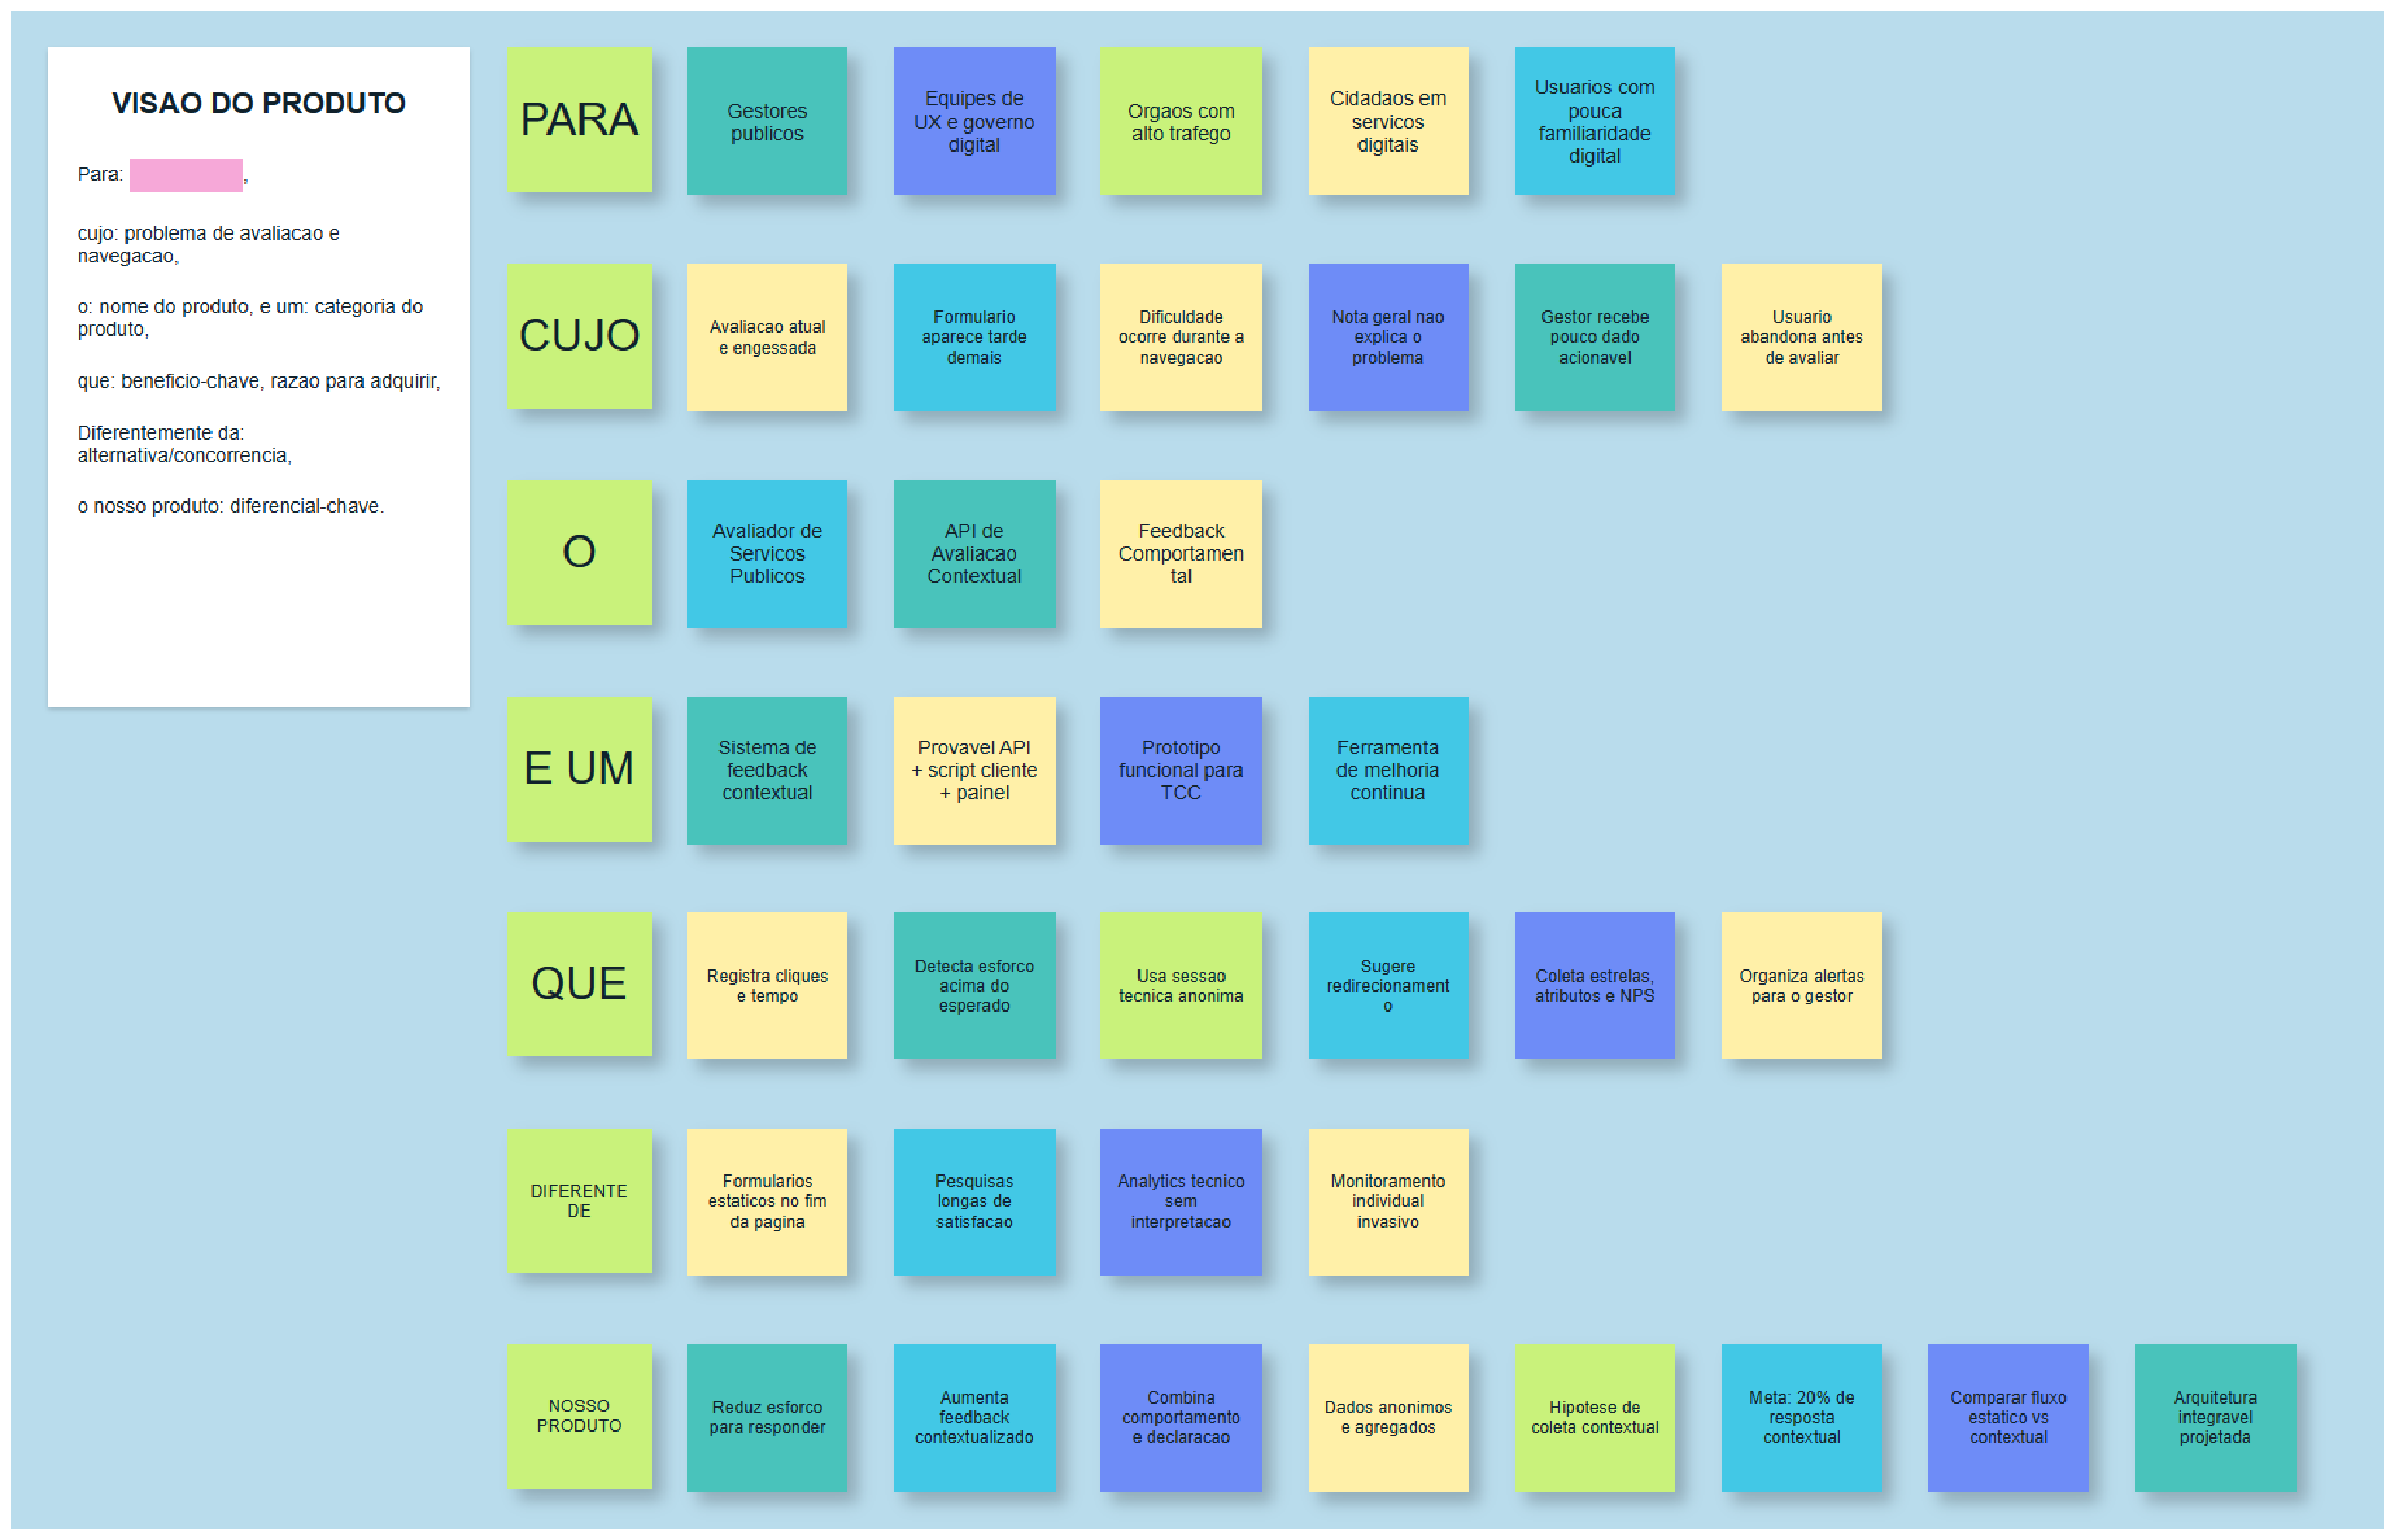
\includegraphics[width=\textwidth,height=0.82\textheight,keepaspectratio]{figuras/apendices/lean-inception-visao-produto.eps}
    \caption{Visão do produto construída na Lean Inception}
    \label{fig:visao-produto-lean-inception}
\end{figure}

A dinâmica É / Não É / Faz / Não Faz delimitou o escopo inicial. O produto é uma
solução técnica real e integrável, demonstrada em ambiente controlado. Também é
um apoio à melhoria de serviços digitais e à decisão administrativa. Não é um
substituto de ouvidoria, não é chatbot, não identifica pessoas e não representa
uma implantação governamental completa. O registro visual dessa definição de
escopo aparece nas Figuras \ref{fig:e-nao-e-faz-nao-faz-1} e
\ref{fig:e-nao-e-faz-nao-faz-2}.

No que faz, o produto registra cliques e tempo de permanência, detecta sinais de
dificuldade, solicita feedback no momento da dificuldade, coleta estrelas,
atributos, NPS e comentário opcional, além de exibir indicadores agregados. No
que não faz, não coleta CPF, nome, e-mail ou login, não rastreia indivíduos
identificáveis, não resolve automaticamente o problema do serviço e não depende
de integração com portais reais para validar o TCC.

\begin{figure}[p]
    \centering
    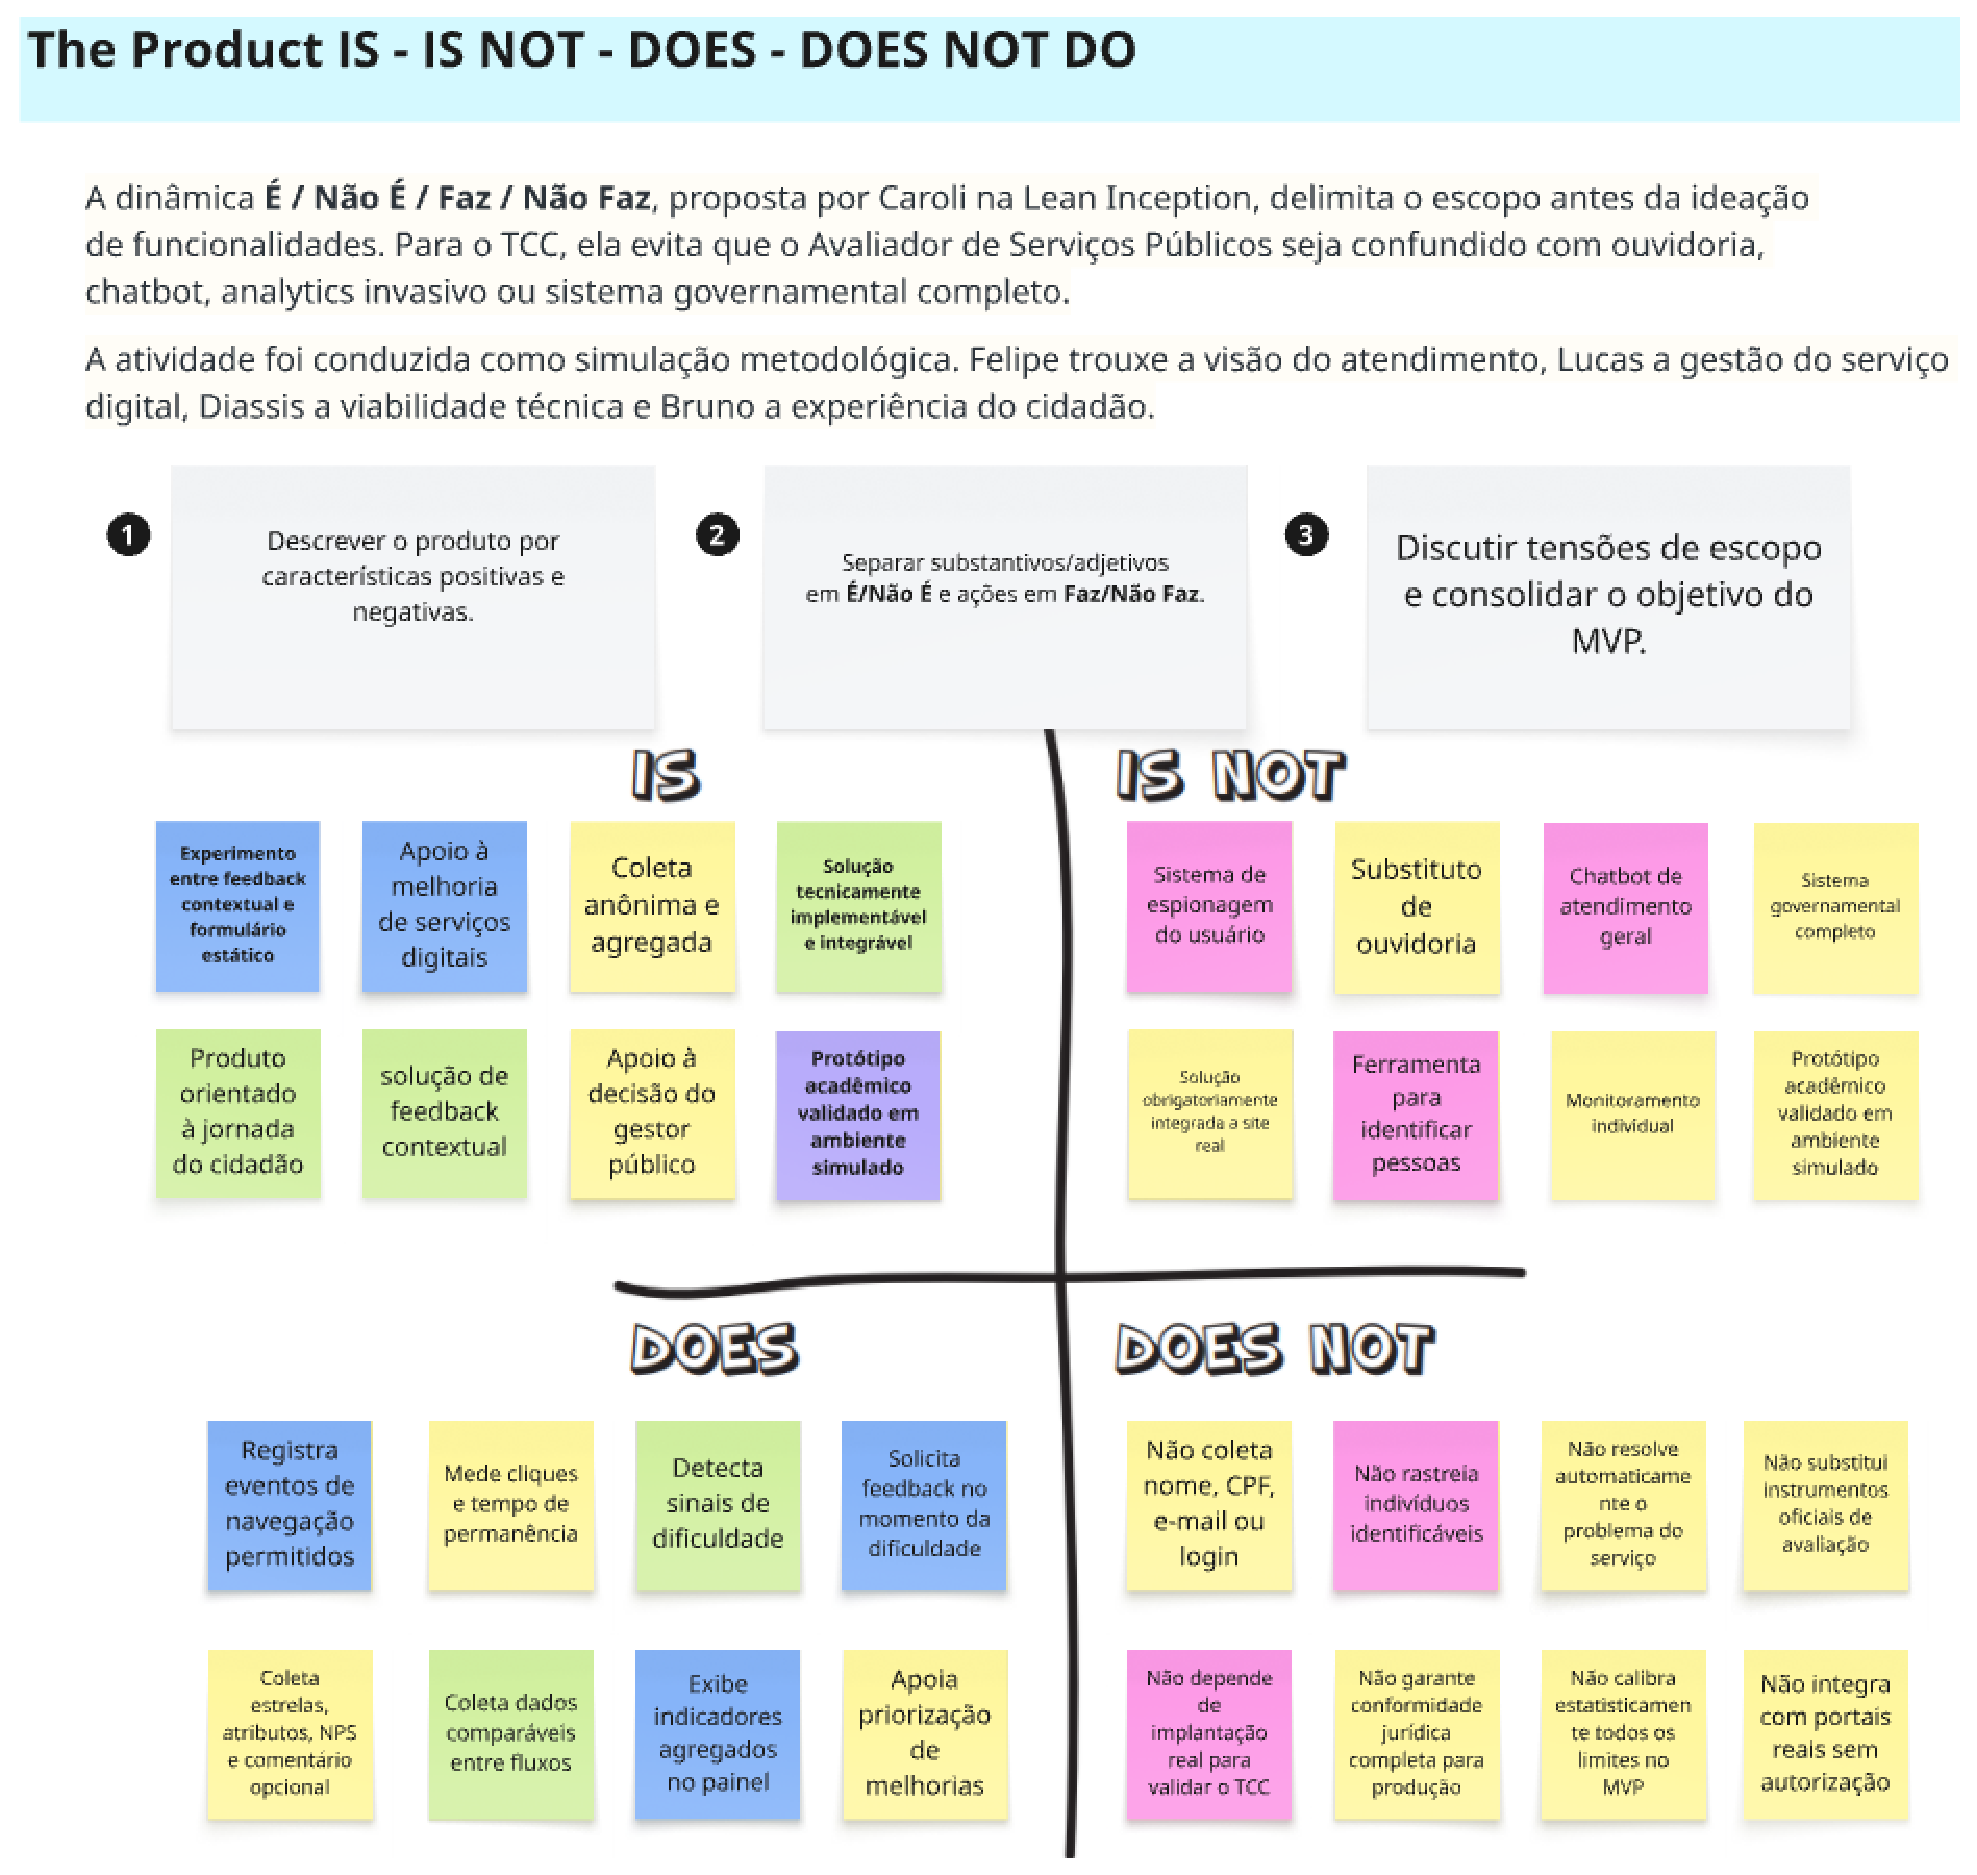
\includegraphics[width=\textwidth,height=0.82\textheight,keepaspectratio]{figuras/apendices/lean-inception-e-nao-e-faz-nao-faz-1.eps}
    \caption{Dinâmica É / Não É / Faz / Não Faz da Lean Inception, parte inicial}
    \label{fig:e-nao-e-faz-nao-faz-1}
\end{figure}

\begin{figure}[p]
    \centering
    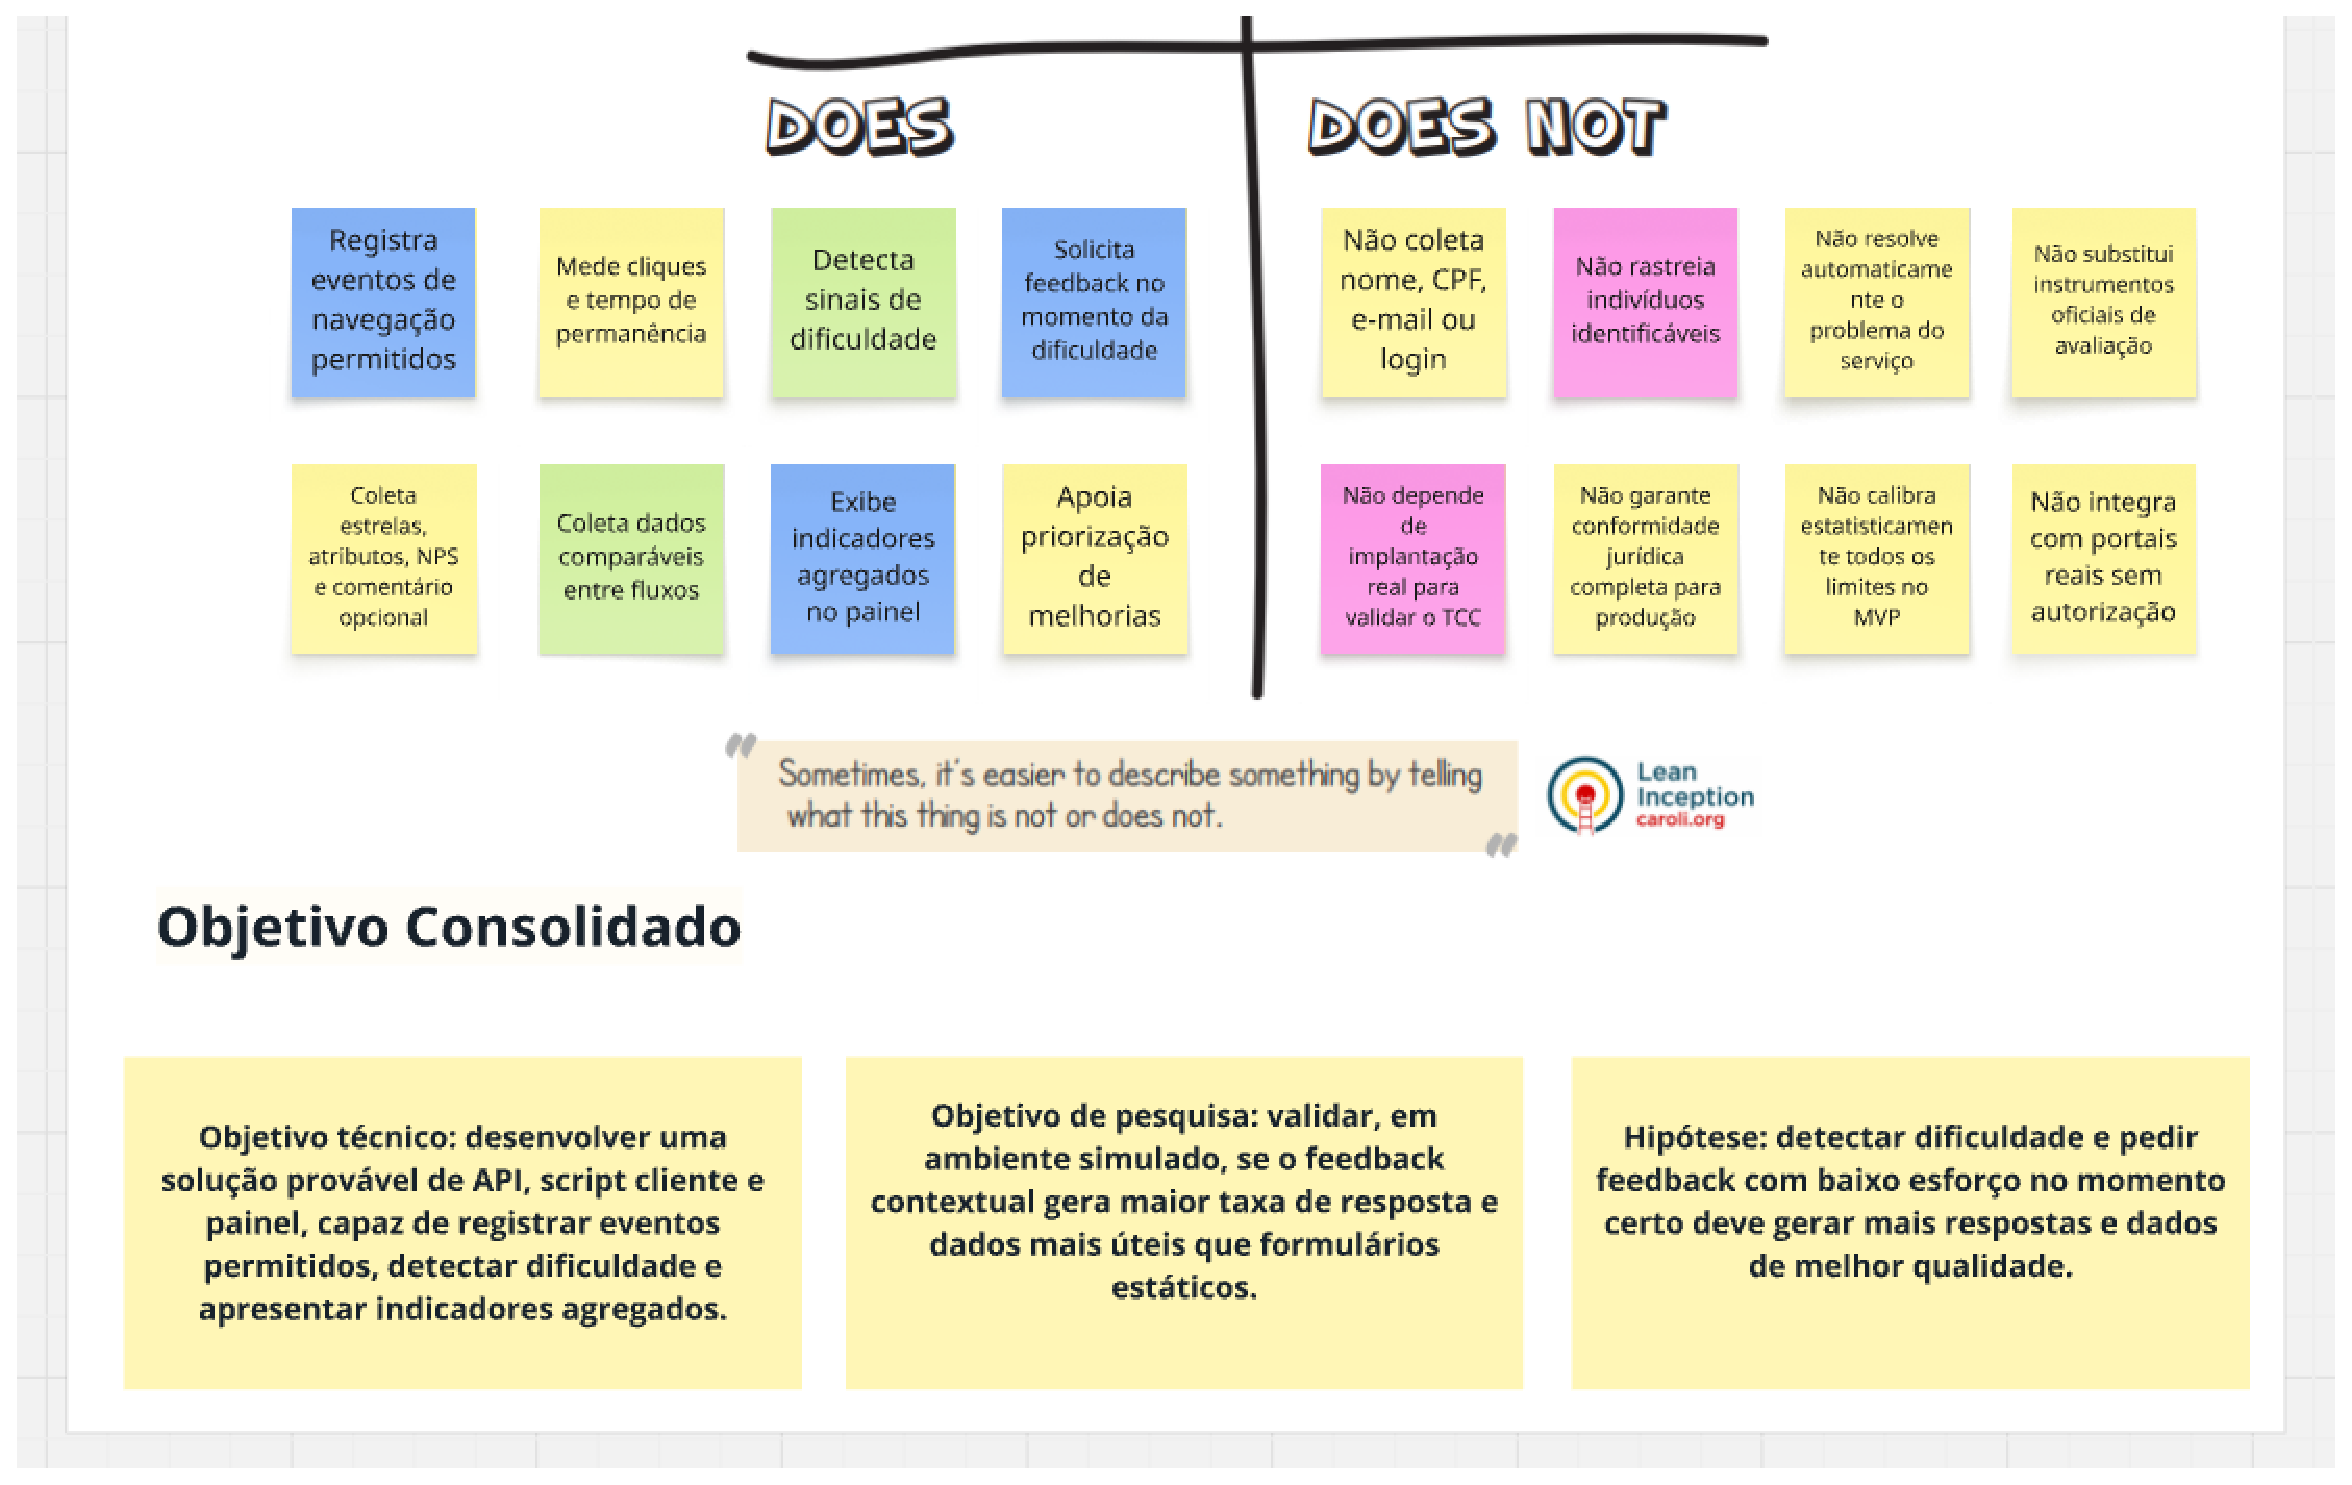
\includegraphics[width=\textwidth,height=0.82\textheight,keepaspectratio]{figuras/apendices/lean-inception-e-nao-e-faz-nao-faz-2.eps}
    \caption{Dinâmica É / Não É / Faz / Não Faz da Lean Inception, continuação}
    \label{fig:e-nao-e-faz-nao-faz-2}
\end{figure}

\clearpage

\section{Objetivos do Produto}

A dinâmica de objetivos do produto separou o que o MVP precisava provar daquilo
que seria apenas evolução futura. Os objetivos levantados foram: capturar sinais
de dificuldade durante a navegação, solicitar feedback no momento adequado,
reduzir o esforço de resposta, gerar dados agregados e acionáveis, coletar dados
comparáveis entre fluxo contextual e fluxo estático, preservar privacidade e
validar o MVP em protótipo controlado.

Foram priorizados três objetivos essenciais. O primeiro é capturar sinais de
dificuldade, pois sem eventos de navegação não há como identificar o momento
adequado para solicitar feedback. O segundo é solicitar feedback contextual, pois
essa é a diferença principal em relação a formulários tradicionais. O terceiro é
coletar dados comparáveis, porque a hipótese do MVP depende da comparação entre
um fluxo estático e um fluxo contextual.

\section{Personas}

As personas representam os usuários e beneficiários da solução. Elas não são os
participantes da Lean Inception; são arquétipos usados para orientar decisões de
produto.

A primeira persona é Carlos Pereira, cidadão usuário de serviço público digital.
Carlos acessa portais públicos para emitir documentos, consultar solicitações ou
encontrar orientações. Ele tem pressa, muitas vezes acessa pelo celular e espera
concluir a tarefa sem entender a estrutura interna do órgão. Suas dores incluem
menus confusos, linguagem institucional, páginas parecidas, excesso de etapas e
avaliações exibidas tarde demais. Seus comportamentos observáveis são cliques
repetidos, permanência acima do esperado, retorno de página, abandono e baixa
disposição para responder pesquisas longas.

A segunda persona é Lucas Almeida, gestor público de serviço digital. Lucas
precisa acompanhar a qualidade de serviços digitais e priorizar melhorias. Sua
dificuldade está em transformar notas genéricas, reclamações isoladas e dados
técnicos em decisões objetivas. Para ele, o produto só gera valor se apontar
onde o cidadão está travando e quais atributos do serviço devem ser priorizados.

A equipe técnica e de UX foi reconhecida como persona secundária de evolução.
Ela seria importante em um piloto real, especialmente para configurar regras,
acompanhar integrações e interpretar dados técnicos, mas não é essencial para
validar o MVP em ambiente de protótipo.

\section{Jornadas}

A jornada principal descreve Carlos tentando usar um serviço público digital.
Ele acessa um portal público, procura um serviço, encontra termos confusos,
clica repetidamente, permanece tempo acima do esperado, tem os sinais registrados
pelo avaliador, recebe feedback contextual e pode responder ou ignorar a
avaliação. Em seguida, os dados são enviados ao painel para que Lucas identifique
um gargalo.

O ponto crítico ocorre entre a dificuldade observada e o abandono da jornada. É
nesse intervalo que o feedback contextual se diferencia de uma avaliação
estática. A proposta é perguntar quando a experiência ainda está recente, sem
exigir um formulário longo e sem interromper a navegação antes de haver evidência
de dificuldade.

Foram definidos dois fluxos comparáveis. No fluxo A, o cidadão navega, enfrenta
dúvidas e recebe um formulário apenas ao final da jornada. No fluxo B, o cidadão
clica ou demora além do esperado, o sistema registra o sinal e solicita feedback
contextual. O painel agrega os resultados para permitir comparação entre taxa de
resposta, qualidade dos dados e identificação de gargalos.

\section{Funcionalidades Priorizadas}

O brainstorming de features agrupou as funcionalidades em cinco categorias:
coleta de sinais, regras e detecção, feedback, painel e integração. A revisão
técnica, de negócio e UX classificou cada funcionalidade por esforço, valor para
gestão, impacto na experiência do usuário e confiança.

A Figura \ref{fig:features-mvp-lean-inception} mostra como as features foram
organizadas antes da seleção do MVP, separando capacidades essenciais de itens
de evolução futura.

\begin{figure}[p]
    \centering
    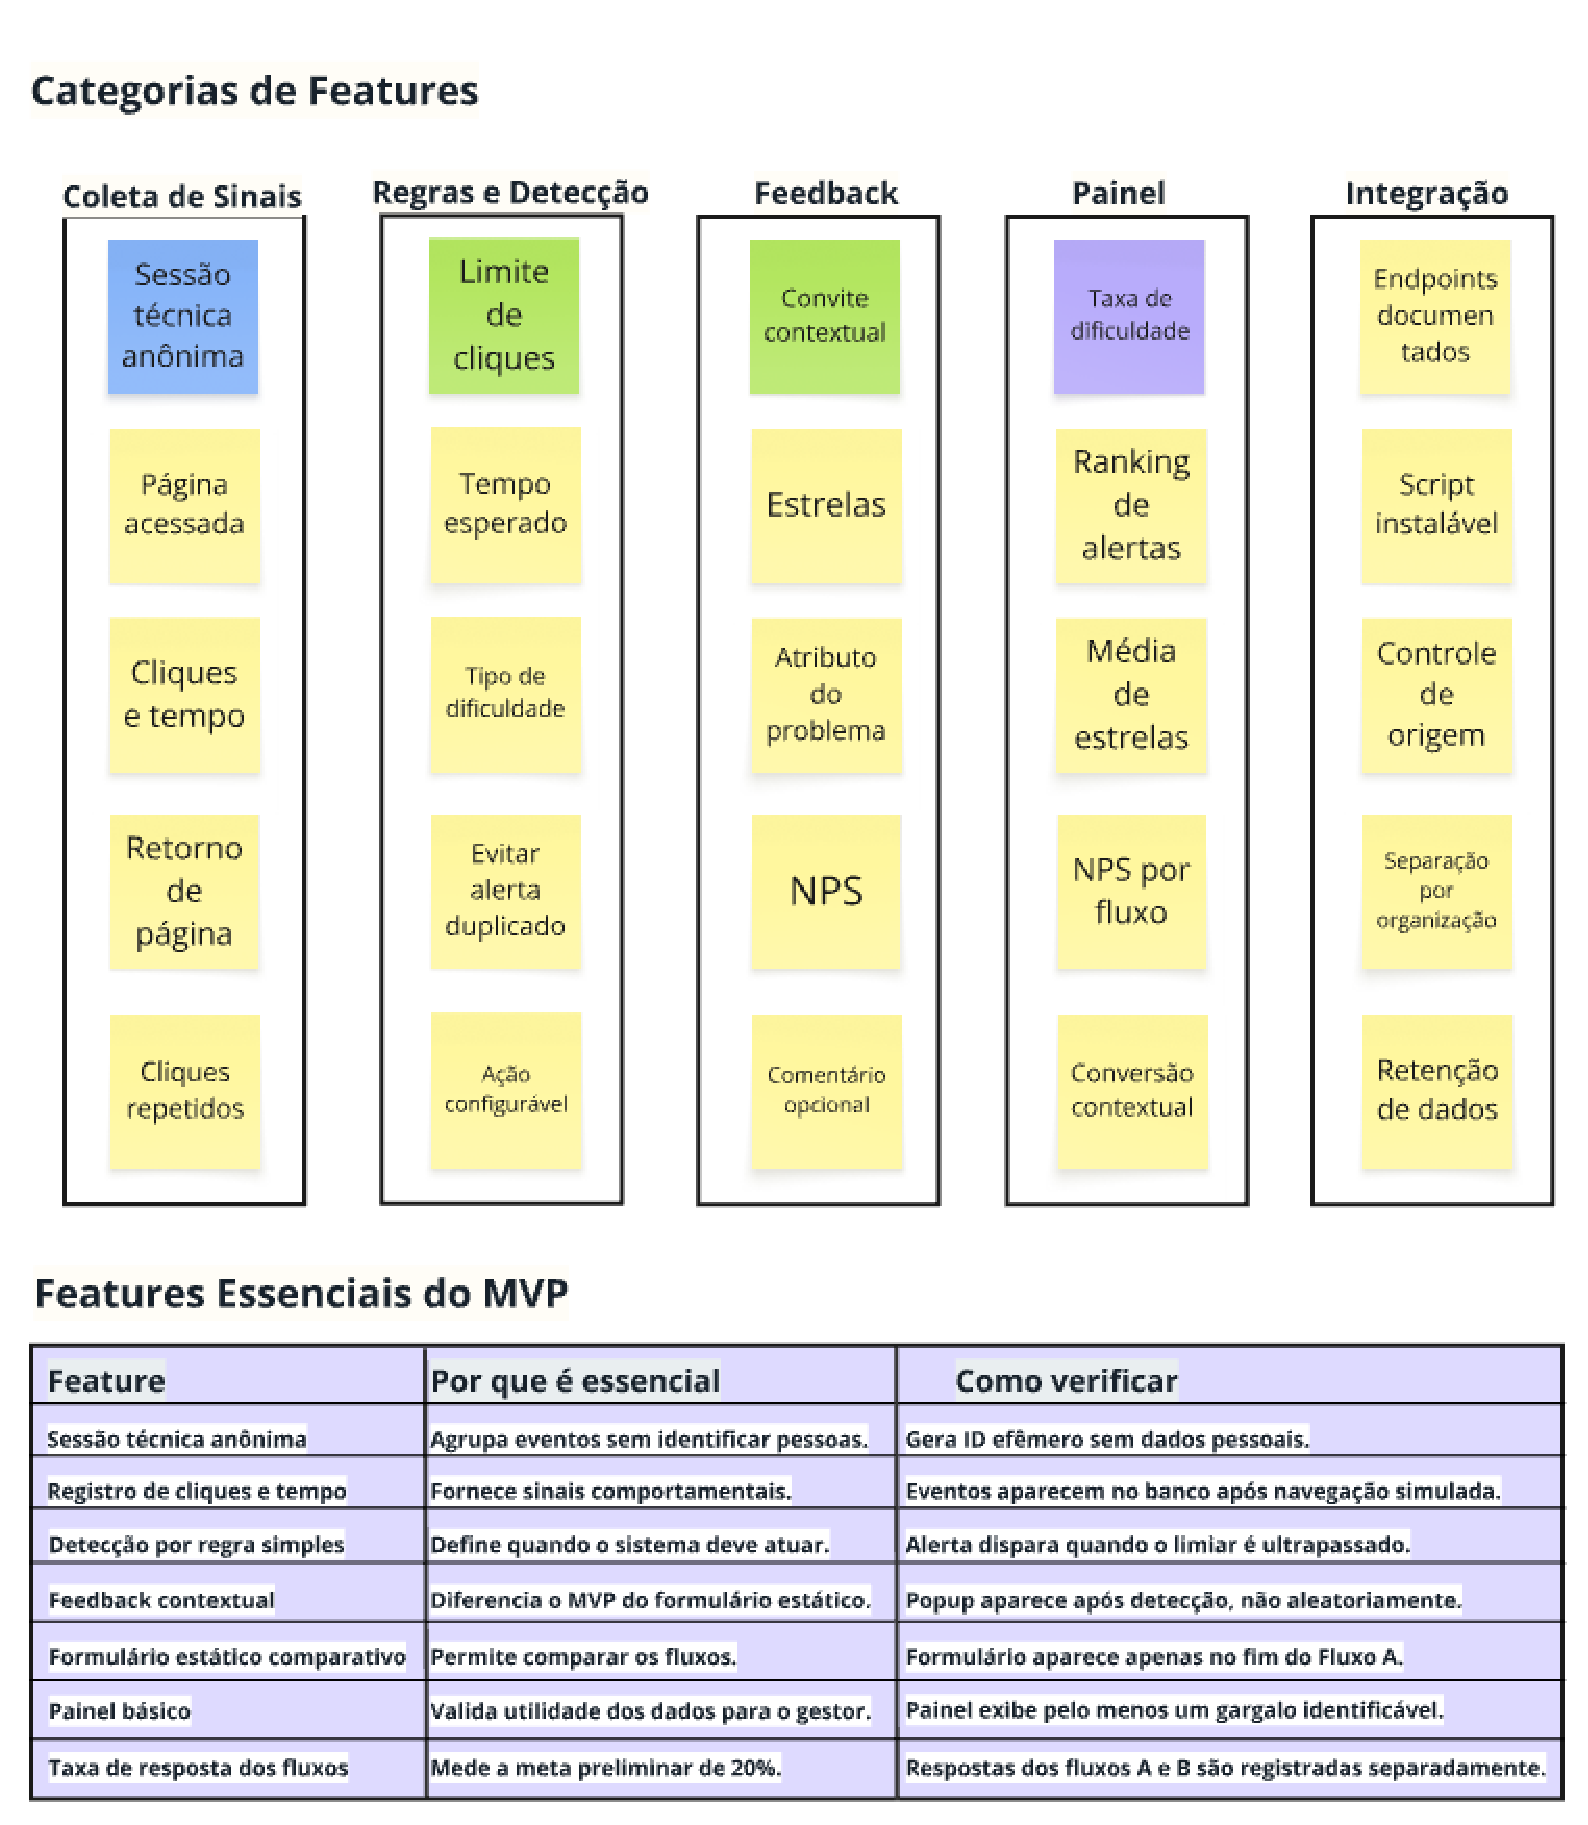
\includegraphics[width=\textwidth,height=0.82\textheight,keepaspectratio]{figuras/apendices/lean-inception-features-mvp.eps}
    \caption{Features categorizadas e essenciais para o MVP}
    \label{fig:features-mvp-lean-inception}
\end{figure}

As funcionalidades essenciais do MVP são:

\begin{itemize}
    \item sessão técnica anônima, para agrupar eventos sem identificar pessoas;
    \item registro de cliques e tempo, para fornecer sinais comportamentais;
    \item detecção por regra simples, para definir quando o sistema deve atuar;
    \item feedback contextual, para diferenciar o MVP do formulário estático;
    \item formulário estático comparativo, para permitir comparação entre fluxos;
    \item painel básico, para validar a utilidade dos dados para o gestor;
    \item taxa de resposta dos fluxos, para medir a hipótese preliminar.
\end{itemize}

Funcionalidades como inteligência artificial para resumir comentários, integração
com portal real, autenticação avançada, separação multi-organização completa e
calibração estatística refinada foram deixadas fora do MVP inicial. Essas
funcionalidades ampliam o escopo técnico e dependem de dados reais, autorização
institucional ou governança de produção.

\section{Sequenciamento e Canvas MVP}

O sequenciador organizou as funcionalidades em cinco ondas. As três primeiras
compõem o MVP: base técnica de coleta, detecção e feedback contextual, e painel
básico para gestão. A quarta onda representa incremento de qualidade, com regras
por serviço, filtros e comentários recentes. A quinta onda prepara evolução para
piloto controlado, com separação por organização, autenticação, chave de API e
script instalável.

O Canvas MVP consolidou a proposta: validar, em ambiente de protótipo, uma
solução contextual, anônima e de baixo esforço para avaliação de serviços
públicos digitais. O resultado esperado é demonstrar que o feedback contextual pode gerar
maior taxa de resposta e dados mais úteis para a gestão do que um formulário
estático exibido apenas no final da jornada.

\section{Arquitetura do Protótipo}

O protótipo foi implementado como uma aplicação local em Python, com servidor
HTTP, banco SQLite e páginas HTML geradas pelo próprio backend. A escolha por uma
estrutura simples reduz dependências externas e facilita a demonstração do fluxo
completo durante o TCC.

A arquitetura possui quatro camadas principais. A primeira é a camada de
interface, composta por uma página inicial de portal público de demonstração,
páginas de serviço, popup de redirecionamento, formulário de feedback e painel visual. A
segunda é o script cliente, responsável por iniciar sessão, registrar eventos de
clique e tempo e enviar dados para a API. A terceira é a API, responsável por
receber eventos, aplicar regras e devolver ações. A quarta é a camada de dados,
armazenada em SQLite.

A Figura \ref{fig:prototipo-portal} mostra a página de portal público usada no
protótipo, incluindo a área lateral que evidencia a comunicação com a API durante
a navegação.

\begin{figure}[htbp]
    \centering
    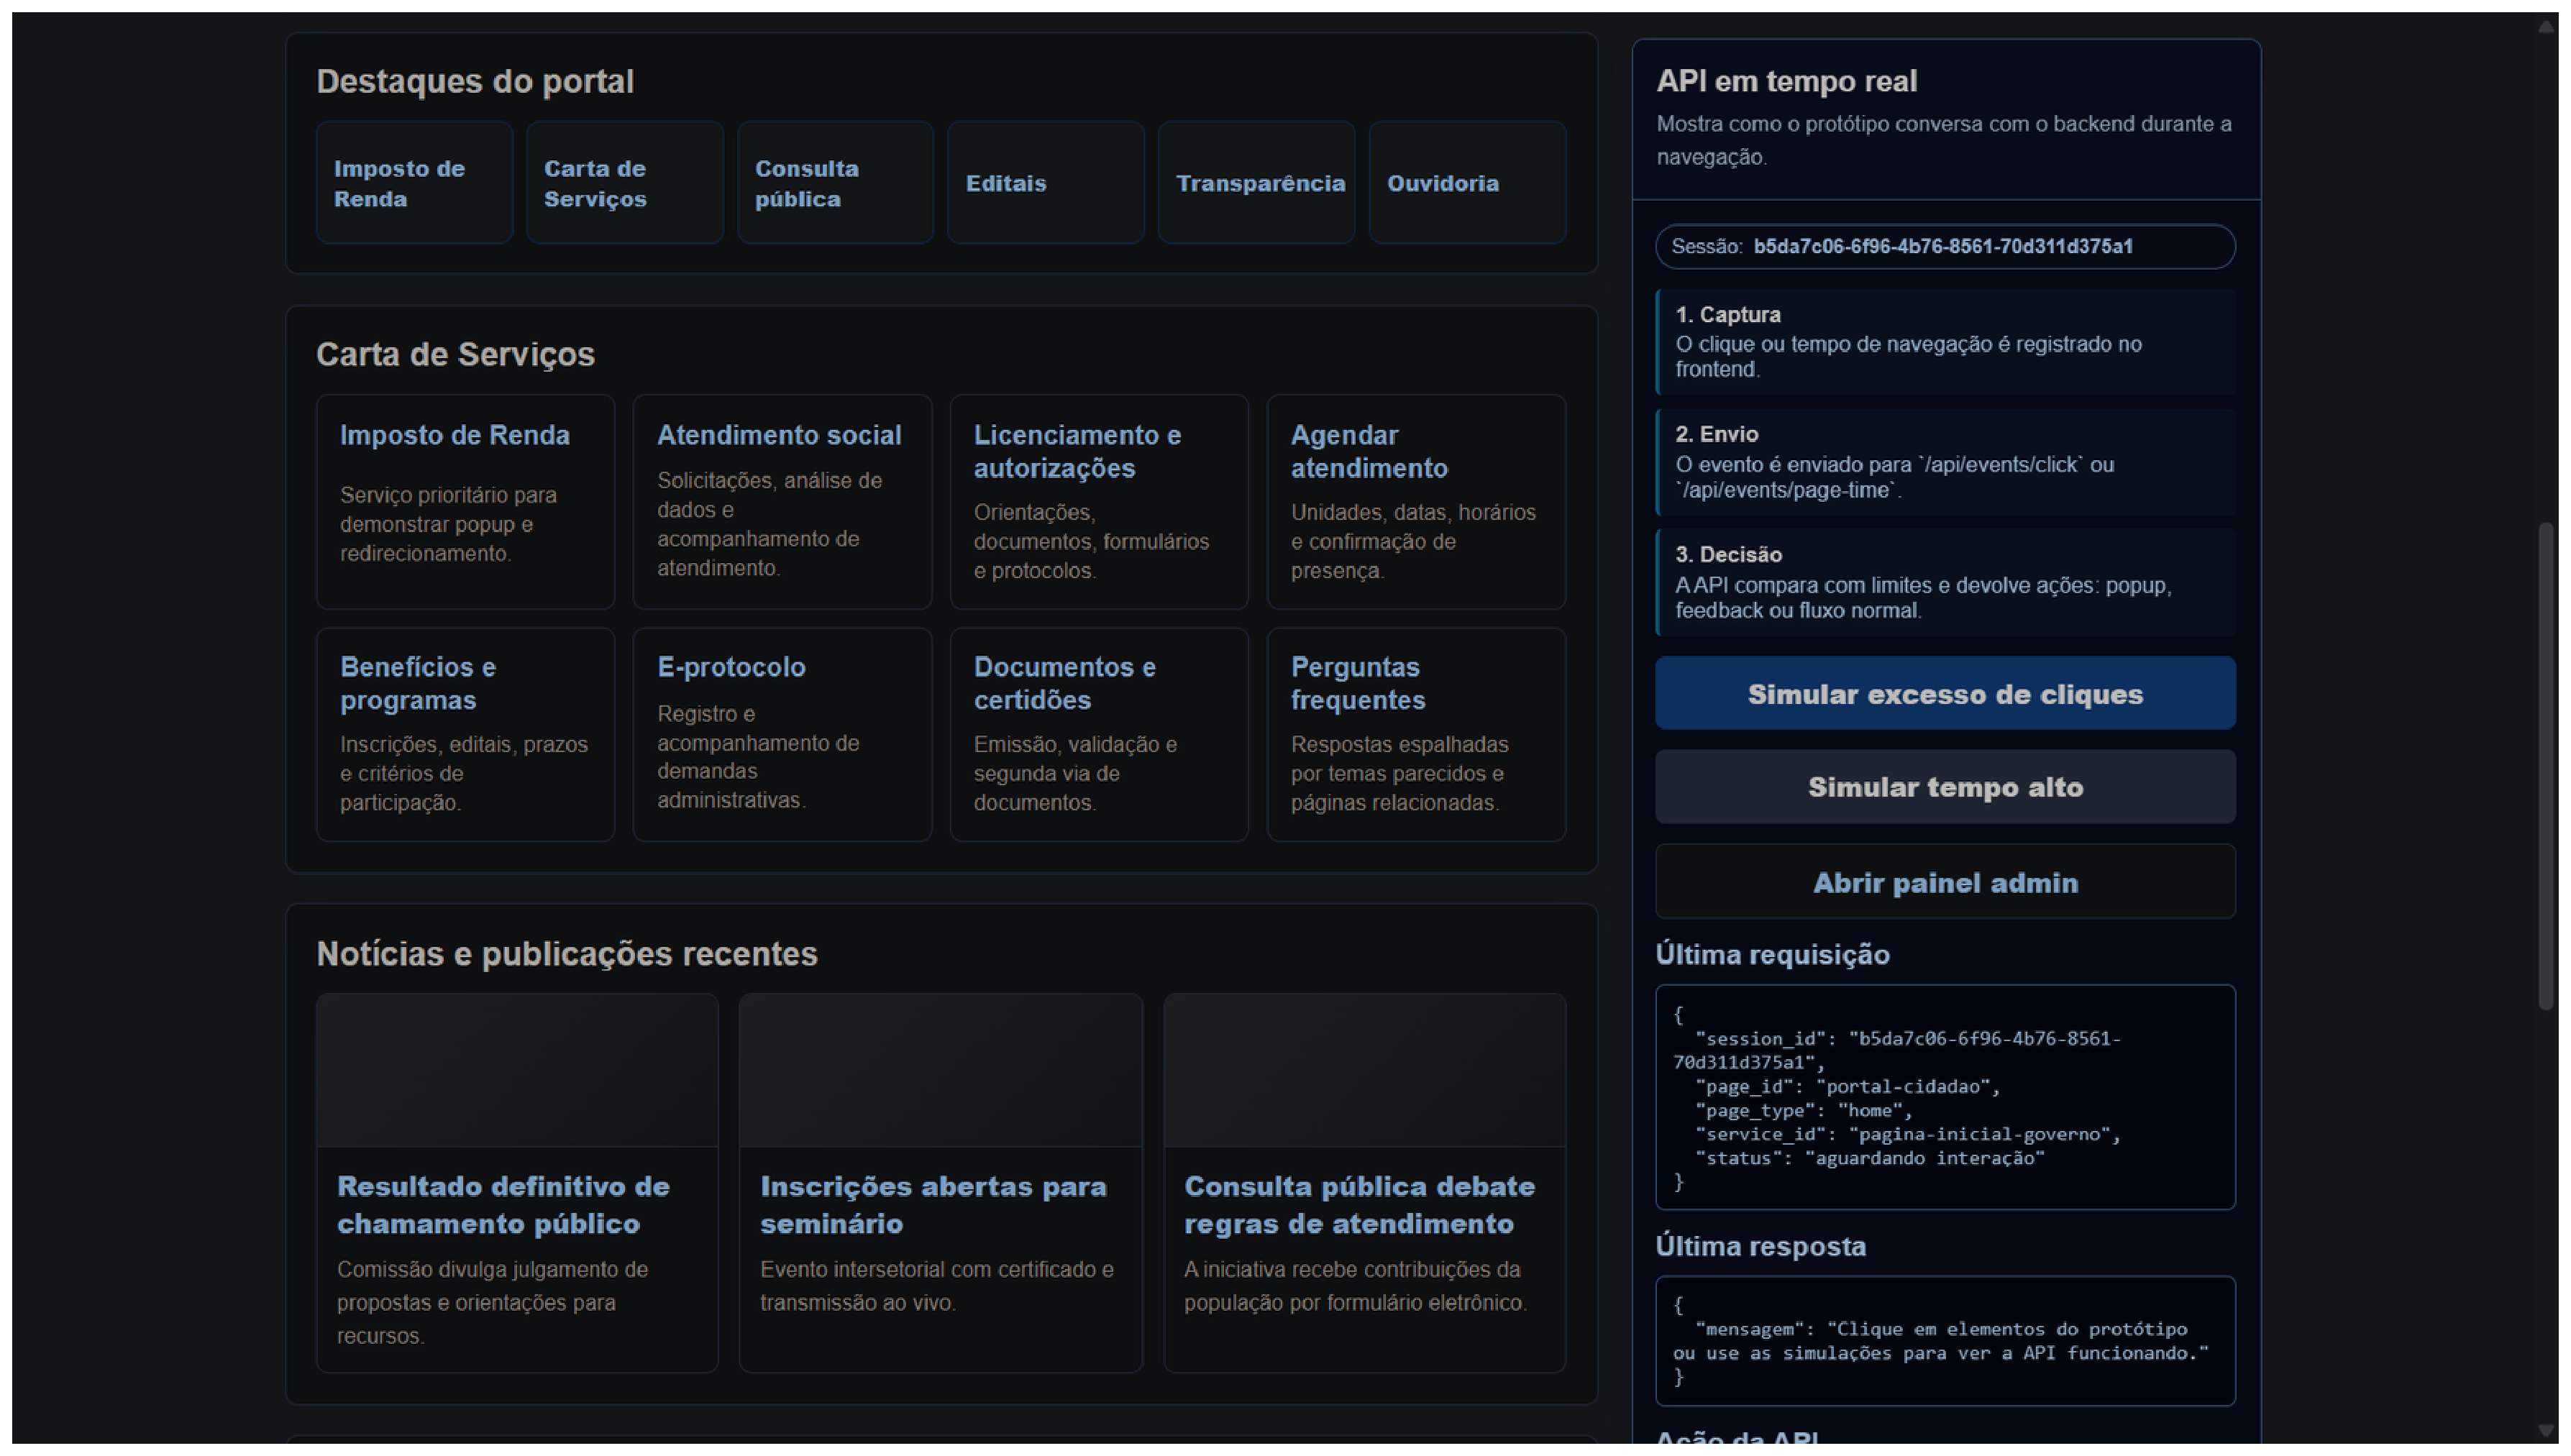
\includegraphics[width=\textwidth,height=0.76\textheight,keepaspectratio]{figuras/apendices/prototipo-portal.eps}
    \caption{Página de portal público usada no protótipo}
    \label{fig:prototipo-portal}
\end{figure}

\clearpage

\section{API e Endpoints}

A API disponibiliza endpoints para saúde do serviço, listagem de serviços,
registro de eventos, envio de feedback e consulta administrativa. O Quadro
\ref{tab:endpoints-prototipo} resume os principais endpoints.

\begin{table}[h]
\centering
\caption{Endpoints principais do protótipo}
\label{tab:endpoints-prototipo}
\begin{tabular}{p{4.2cm} p{8.4cm}}
\hline
\textbf{Endpoint} & \textbf{Finalidade} \\
\hline
\texttt{GET /health} & Verificar disponibilidade da API. \\
\texttt{GET /api/services} & Listar serviços cadastrados e suas regras. \\
\texttt{POST /api/events/click} & Registrar clique, página, serviço, origem e
instante. \\
\texttt{POST /api/events/page-time} & Registrar tempo de permanência em página
ou serviço. \\
\texttt{GET /feedback} & Exibir página simples de feedback para uma sessão. \\
\texttt{POST /api/feedback} & Salvar estrelas, atributos, NPS e comentário. \\
\texttt{GET /api/admin/alerts} & Consultar alertas silenciosos de dificuldade. \\
\texttt{GET /api/admin/dashboard} & Consultar dados agregados para o painel. \\
\hline
\end{tabular}
\end{table}

\section{Regras de Detecção de Dificuldade}

A detecção de dificuldade foi implementada com regras explícitas no backend. A
API mantém, para cada serviço, um limite de cliques e um tempo médio esperado. Um
alerta de dificuldade por clique é criado quando a contagem de cliques da mesma
sessão, no mesmo serviço, fica \textbf{maior} que o limite configurado. Um alerta
de dificuldade por tempo é criado quando a permanência informada fica
\textbf{maior} que 1,5 vez o tempo médio do serviço.

Essas regras operacionalizam o conceito de feedback contextual discutido na
Seção~\ref{sec:feedback-contextual}: o sistema não pergunta aleatoriamente, mas
usa sinais de uso para decidir quando a coleta tem maior chance de representar
uma dificuldade real.

No protótipo atual, as regras são as seguintes:

\begin{table}[h]
\centering
\caption{Regras de detecção de dificuldade no protótipo}
\label{tab:regras-dificuldade}
\begin{tabular}{p{3.6cm} p{3.0cm} p{2.4cm} p{4.2cm}}
\hline
\textbf{Serviço} & \textbf{Cliques} & \textbf{Tempo} &
\textbf{Ação principal} \\
\hline
Página inicial do governo & a partir do 13\textsuperscript{o} clique &
mais de 90 segundos & recomenda Imposto de Renda e, com dificuldade persistente,
abre feedback \\
Imposto de Renda & a partir do 11\textsuperscript{o} clique; feedback no
12\textsuperscript{o} clique & mais de 67,5 segundos & exibe popup de
redirecionamento e pode abrir feedback \\
Serviço público genérico & a partir do 13\textsuperscript{o} clique &
mais de 90 segundos & abre feedback sem popup
prioritário \\
\hline
\end{tabular}
\end{table}

\clearpage

A página inicial do governo é tratada como contexto capaz de recomendar um
serviço prioritário. O serviço de Imposto de Renda foi marcado como importante e
de alto tráfego. O serviço genérico representa uma situação comum, na qual a API
registra a dificuldade e pode abrir feedback sem sugerir redirecionamento. Em
todos os casos, o alerta administrativo é silencioso: o cidadão não precisa saber
que a sessão foi marcada como difícil, mas o gestor passa a visualizar o evento
no painel.

\section{Fluxos Implementados}

O fluxo de clique começa quando o usuário acessa uma página simulada. O script
cliente cria ou recupera uma sessão técnica anônima, captura o evento e envia os
dados para a API. A API registra o clique, atualiza a contagem por serviço,
verifica o limite configurado e decide se deve retornar fluxo normal, popup de
redirecionamento ou convite de feedback.

Quando o serviço é prioritário, a API pode retornar uma ação de popup sugerindo
redirecionamento para o serviço correto. Esse popup é exibido apenas uma vez por
sessão, serviço e motivo, evitando repetição excessiva. Quando a dificuldade
continua ou quando o tempo de permanência ultrapassa a faixa esperada, a API pode
retornar uma ação para abrir o feedback.

O fluxo de feedback coleta avaliação por estrelas, características do problema,
NPS e comentário opcional. As características previstas incluem clareza, tempo,
esforço, usabilidade, atendimento e eficácia. O objetivo é transformar uma nota
geral em dados explicativos para o gestor.

A Figura \ref{fig:prototipo-feedback} apresenta a tela de feedback contextual,
com avaliação por estrelas, atributos do problema, NPS e comentário opcional.

\begin{figure}[htbp]
    \centering
    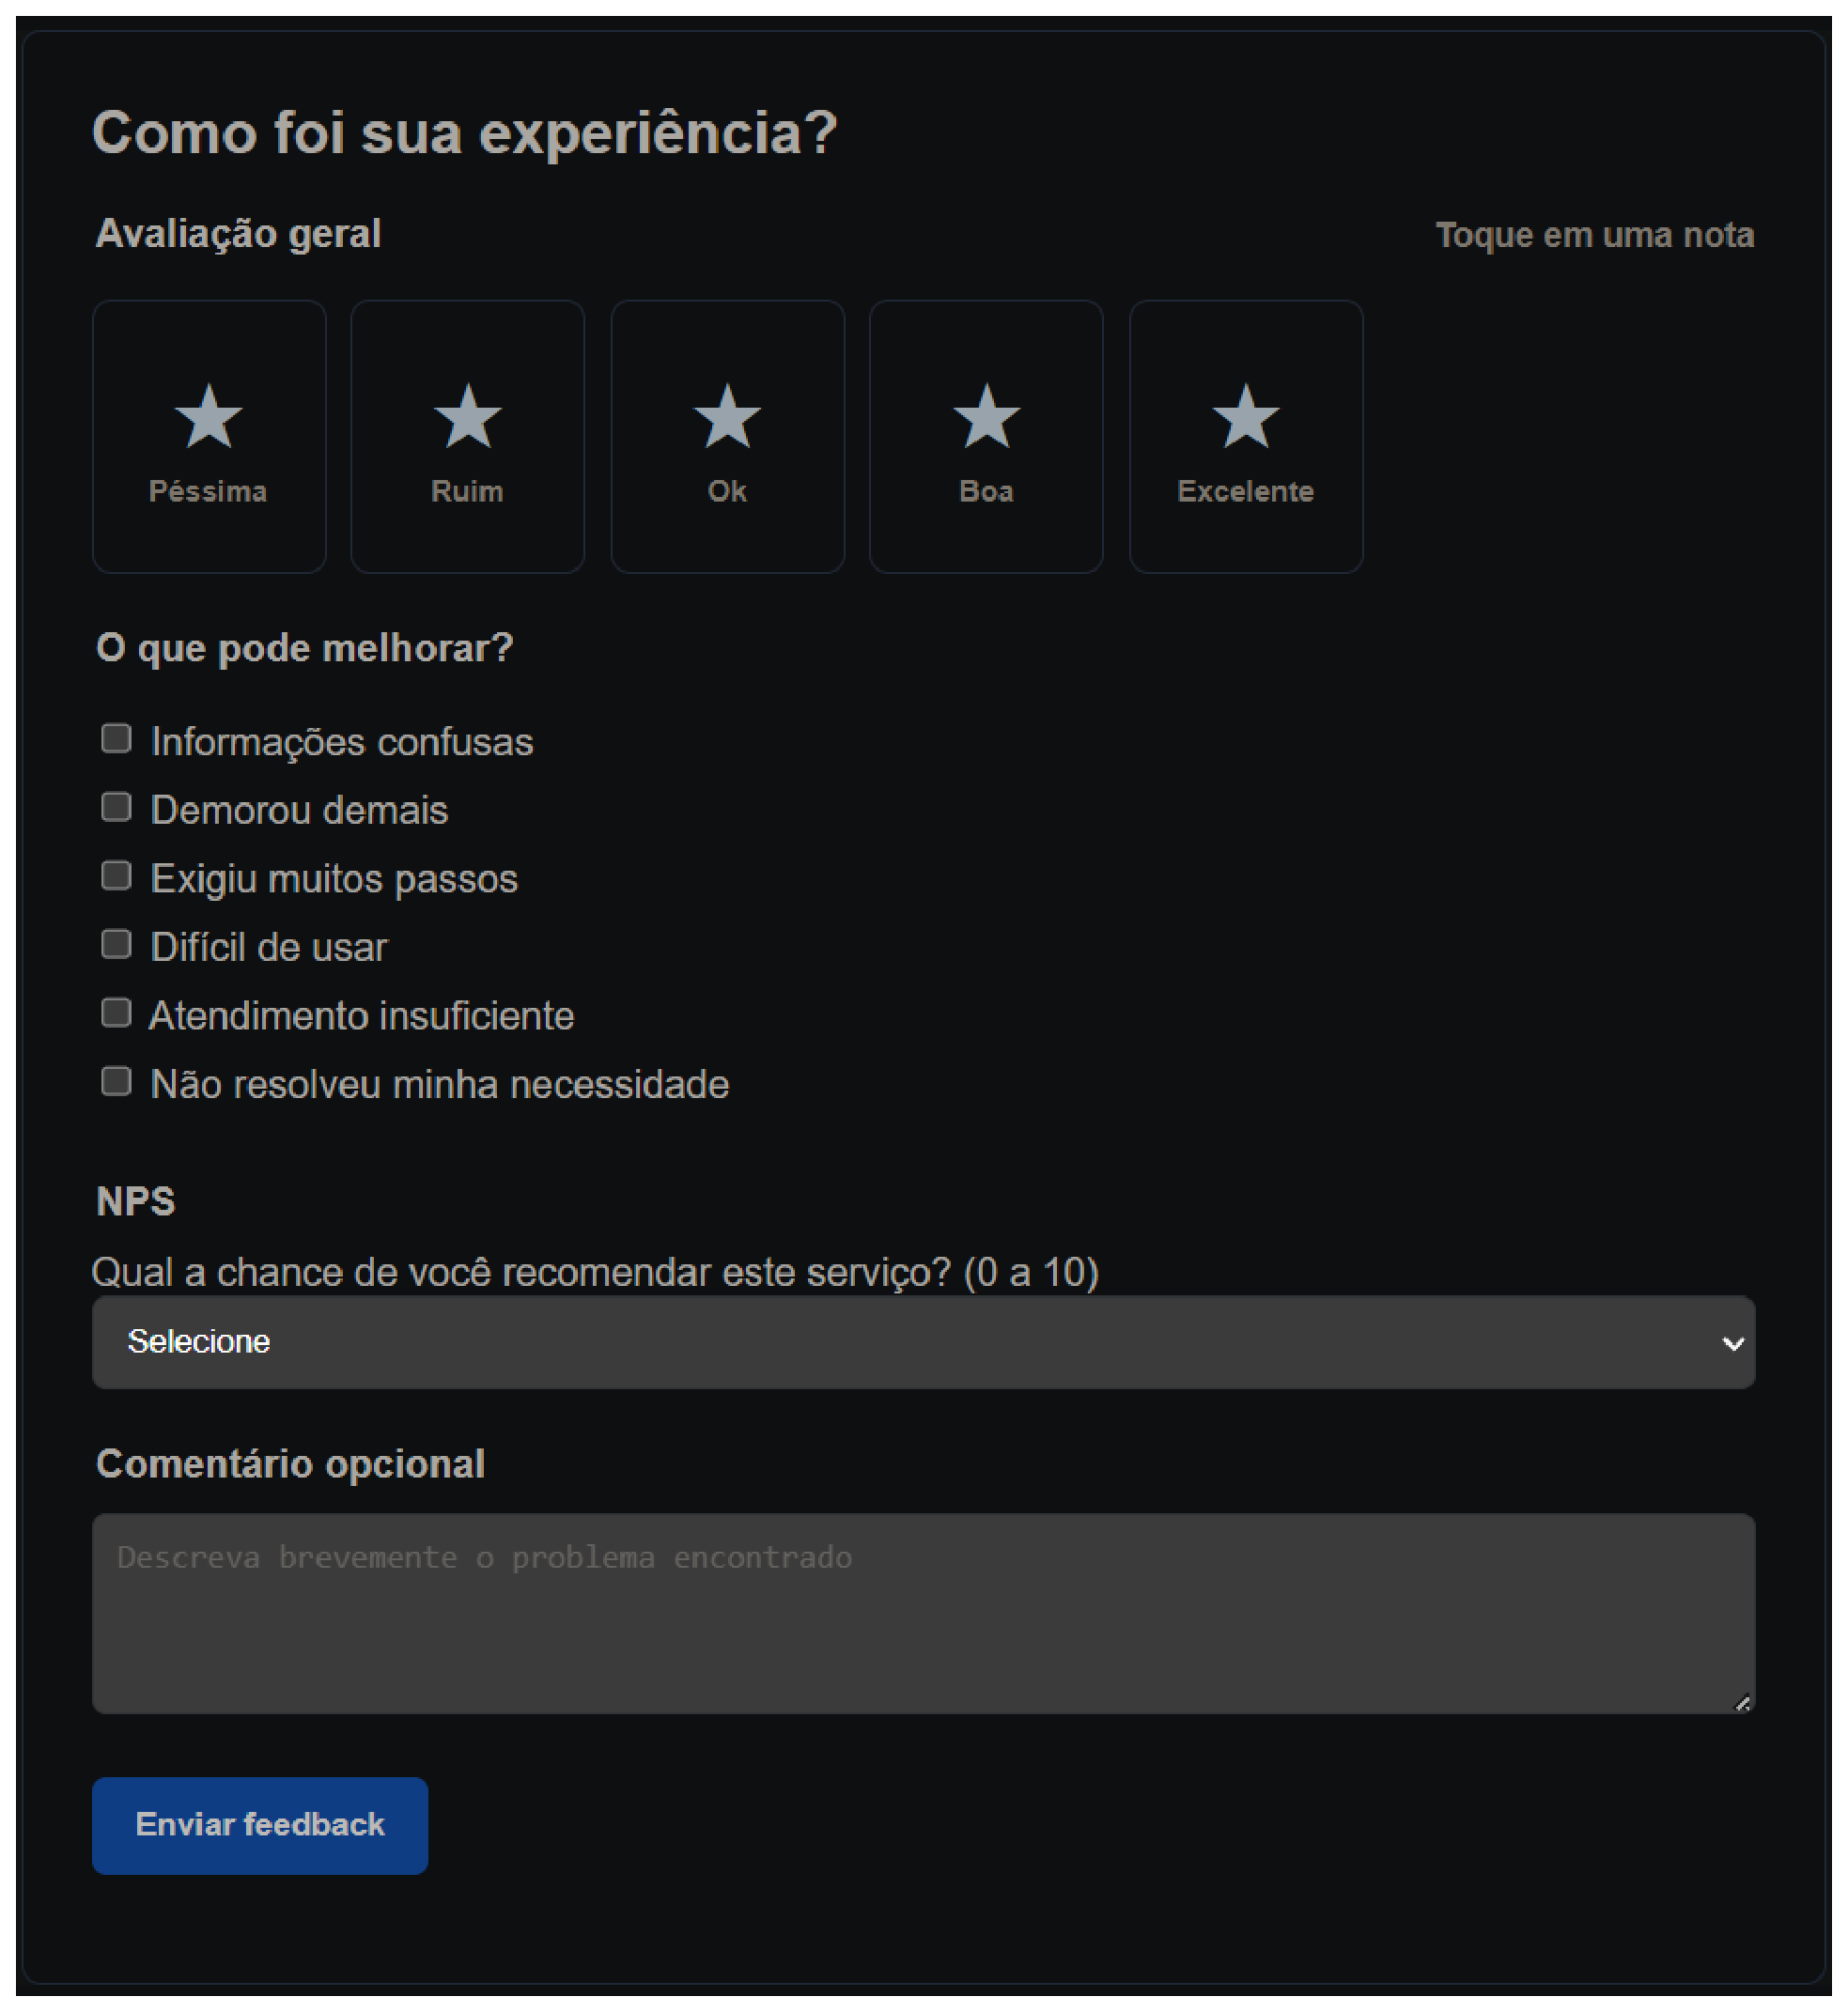
\includegraphics[width=\textwidth,height=0.76\textheight,keepaspectratio]{figuras/apendices/prototipo-feedback.eps}
    \caption{Formulário de feedback contextual do protótipo}
    \label{fig:prototipo-feedback}
\end{figure}

\clearpage

\section{Painel Administrativo e Indicadores}

O painel administrativo apresenta alertas e métricas agregadas. Os principais
indicadores previstos são total de alertas, sessões com dificuldade, serviços
com maior recorrência de alertas, média de estrelas, total de feedbacks, NPS e
atributos mais selecionados. Esses dados permitem que o gestor identifique
gargalos demonstrados, como excesso de cliques em um serviço específico ou
recorrência de problemas de clareza.

A análise não pretende substituir instrumentos oficiais de avaliação. Seu papel é
complementar a avaliação tradicional com evidências de contexto: onde a
dificuldade ocorreu, qual serviço estava associado, qual foi o tipo de sinal e
qual feedback foi declarado pelo cidadão.

\section{Resultado do Desenvolvimento}

O desenvolvimento resultou em um protótipo funcional capaz de executar o fluxo
central definido na Lean Inception. O usuário navega por páginas públicas
simuladas, a API registra eventos, regras identificam dificuldade, o feedback é
solicitado de forma contextual e os dados aparecem no painel administrativo.

O protótipo também materializa a comparação proposta entre fluxo A e fluxo B. O
fluxo estático representa a avaliação ao final da jornada; o fluxo contextual
representa a avaliação acionada por sinais de dificuldade. A comparação ainda
precisa de testes com participantes, mas a solução já fornece a estrutura técnica
para coletar os dados necessários.
